\chapter{Background}\label{sec:Background}
In this section we will go over some of the fundamentals of distributed systems and algorithms that will help to better understand the later parts of this report.

We will first give a brief introduction to the main challenges of working in distributed environments. Then we will discuss a fundamental problem of distributed systems known as Consensus, followed by the description of one of the most popular algorithms used to solve Consensus in distributed settings, called Paxos. Lastly we will introduce GeoPaxos, an improvement over Paxos which aims to provide better performance in geo-distributed environments.

\section{Distributed Systems}\label{sec:Distributed Systems}

Distributed systems can be encountered in a multitude of situations in our everyday lives, and their importance is growing every year: Entertainment services such as music and video streaming services, banks, hospitals, social medias, web engines are just a few of the many types of distributed systems that we use on a daily basis, and each of these may have different challenges and needs when it comes to handling distribution.

Even a clear definition of a distributed system is hard to find. In general, we can describe it as a collection of indipendent machines that communicate and coordinate their work to provide a certain service to its users: to them, the system should appear as a single and homogeneous entity, hiding its distributed nature.

Working with distributed environments has some inherent challenges, some more important than others depending on the specific system. Concurrency issues, for example when multiple users want to withdraw money from a bank account. Ordering and synchronization, because the different machines will most likely work with different clocks and their communication may take a noticeable amount of time. Failure resiliance, so that the system does not go down when one of its machines fails. These are only a few of the many problems that can and will be encountered when working with distributed systems.

To tackle these problems, The choice of the models used to represent them is fundamental: choosing a model too strong may make the problem easier to solve, but it may represent an unrealistic view of the problem at hand. On other hand, weaker models may make the problem impossible to solve without further assumptions. 

A synchronous system is one where we know that the process speed and the time delay for the communication are bounded; this helps us simplify our view of the timing and communication side, but it will usually not be a realistic representation of the real world system.

On the other hand, an asynchronous system is one that  does not have bounds on process speed and time delay, which is a more general assumption which could greatly increase the difficulty of solving the problem.

Similarly, for a model we could have reliable channels, where if a process sends a message and the receiver does not crash then the receiver will get the message, or quasi-reliable, where both sender and receiver must not crash for the receiver to get the message.

It is also important to model the possible failure of the processes. 
Some types of failure models can be:
\begin{itemize}
\item \textbf{Failstop} the process fails by halting execution, and it does not recover. Other processes will know about the failure of the process
\item \textbf{Crash} the process fails by halting execution, and it does not recover. Furthermore, the other processes may not be able to identify its failure
\item \textbf{Byzantine failures} the process fails by exhibiting arbitrary behavior, which could be unexpected replies or malicious actions
% \item \textbf{Crash+Link} a link fails by losing some messages, but does not delay, duplicate, or corrupt messages.
% \item \textbf{Receive-omission}: a process fails by receiving only a subset of the messages sent to it, or by halting (i.e., crashing).
\end{itemize}

Again, the choice of the failure model gives us different degrees of difficulty: a failstop model makes the problem easier to solve, but a system that is able to tolerate byzantine failures is going to be much more resiliant to failures.

\section{Consensus}\label{sec:Consensus}

The problem of consensus is a fundamental problem in distributed systems: it was first introduced in the early 80s \cite[]{Pease}, \cite[]{Lamport} and since then it remained important in most distributed environment, ranging from more classical server applications to the more recent Blockchains.

Consensus is basically an agreement problem: the goal is to have a set of entities reach an agreement on a value that was previously proposed by (at least) one of those entitities. This definition is quite general, and for a good reason: depending on the different assumptions we make on the system model, there are stronger and weaker types of consensus that can be achieved. 

The three core properties of a consensus protocol are the following:

\begin{itemize}
    \item \textbf{Termination} Eventually every correct process decides on one value
    \item \textbf{Uniform integrity} If a process decides on a value, then this value was proposed by some process
    \item \textbf{Uniform agreement} No two processes decide on a different value
    \end{itemize}

\begin{figure}[htb]
  \centering
  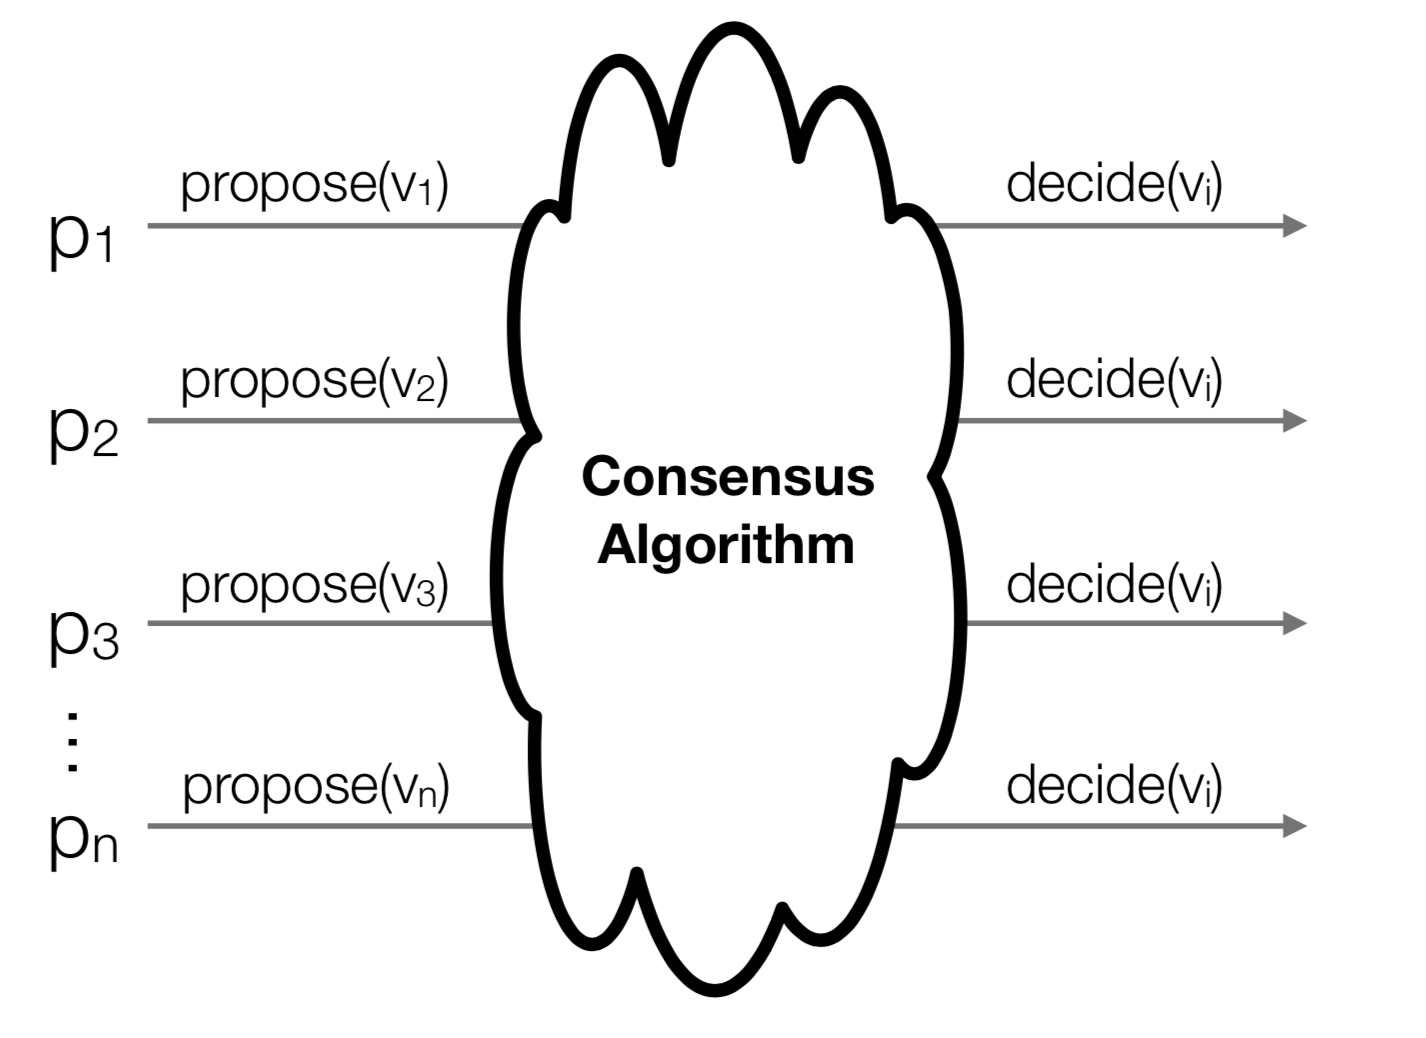
\includegraphics{img/consensus.png}
  \caption[The architecture of the system]{ The architecture of the system. The
    \textit{Viper IDE} and \textit{Viper Debugger} boxes denote, respectively,
    the main Viper extension and the new debugger extension. They both interact,
    independently, with Visual Studio Code. Viper Server is responsible for
    running the verification backends.}
  \label{fig:consensus}
\end{figure}

In this section we will go over some of the more relevant types of consensus, and respective implementations that are able to achieve consensus in the given system models.


\subsection{Synchronous model}\label{sec:Synchronous model}
In a synchronous system model, consensus is quite straightforward to achieve. Let us assume to have a set of $n$ processes, that will be the entities that want to reach a common agreement upon a proposed value. Let us also introduce the primitives used by the processes: each process is able to send and receive messages, through the primitives $send(m)$ and $receive(m)$ respectively, to communicate their intentions to the others. The failure model in a crash failure model, hence a correct process will never crash, while a faulty one eventually will; the number of faulty processes $f$.

Since we are in a synchronous model, we have a bound on the maximum time delay of a message, which means that a process is sure that if a message is sent, it will be received by the receiver before the maximum time delay. This is a quite strong and unrealistic model, but it makes the algorithm to solve consensus quite simple.

Let us have the algorithm proceed in rounds, where each round is as follows:
\begin{enumerate}
    \item Each process sends to all other processes a message containing information about its state.
    \item At the end of the round, after the maximum time bound, processes will have received a set of messages from a subset of all processes.
    \item The processes will then use the received messages together with its current state to reach a new state.
\end{enumerate}

The state can be simply a set values received until that moment, with the initial set containing only our own proposed value. Also, in a round a process can receive only a subset of messages from the other processes, since we can have up to $f$ faulty processes.

After $f+1$ rounds, we can be certain that each correct process will have enough information to deterministically decide on a single proposed value, and therefore reach consensus. This is because if we have a round where no process fails, then every process will receive all other values, and therefore we will be able to decide on a value. Also, since we have at most $f$ faulty processes, we can have at most $f$ rounds with a failing process. Therefore, we can be certain that $f+1$ rounds will be enough to reach agreement.

[should I put the lemmas properly?]

\subsection{Asynchronous model}\label{sec:Asynchronous model}
In this model, we have no bounds on process speed and maximum message delays; this means that a process if or when a message will be received by the other processes. This is a much weaker model compared to the previous one, and as a matter of fact it is proven that consensus cannot be solved in such a model [FLP proof].

\subsection{Alternative models}\label{sec:Alternative models}
The synchronous model allows us to solve consensus, but it's too strong of a model to be of any practical use. The asynchronous model cannot solve consensus. Therefore, we either have to find a system model that is weaker than synchronous and stronger than asynchronous, or we have to weaken the problem.

An alternative system model would be a partially-synchronous one, where the messages are asynchronous up to a GST (Global Stabilization Time), after which we can assume communication to become synchronous.

Another option is to still use an asynchronous system, but to also elect a process to be the leader and guide the whole decision procedure; an example of such an algorithm is Paxos, which is presented in the next section.

We could have failure detectors (which can be used with varying levels of completeness and accuracy), which could allow us to figure out when a process has failed, and therefore stoping us from waiting indefinitely for a message like in the basic asynchronous model.

An example of weaker problem definition would be to allow, for example, to have multiple values decided.

\section{Paxos}\label{sec:Paxos}
Paxos is an algorithm to achieve consensus that relies on an asynchronous system model, which makes it particularly interesting for real world application where we don't have completely reliable communication channels. To achieve this, the Paxos algorithm needs to elect one process as a leader that will act as a coordinator during the various phases of the protocol.

In Paxos, there are four types of process roles:
\begin{itemize}
  \item \textbf{Proposers} the processes that want to propose a value to be decided
  \item \textbf{Acceptors} the processes that take part in the voting part of the protocol; a quorum of acceptors is needed
  \item \textbf{Learners} the processes that, at the end of the algorithm, will be notified about the value decided by the algorithm
  \item \textbf{Leader} the process that acts as a coordinator
\end{itemize}

The election of the leader can be achieved in many different ways, as long as there is a point after which we have a unique correct process that is identified by the other processes as the leader.

The algorithm is divided into tree phases. During phase 1, a proposer that wants to propose a new value sends a new arbitrary value c-rnd higher than any previous c-rnd to the acceptors, so that all of them know that this is the most recent proposal attempt. Each acceptor, if the received c-rnd is truly the highest one it has received, replies to the proposer with its current state (rnd, v-rnd, v-val) so that the proposer know if there was already a previous proposed value, or if the proposer is allowed to propose its own.

In phase 2, once the proposer has received a reply from a quorum of acceptors, it checks if there was any acceptor that had previously voted for a value, and if this is the case, it picks the most recent one as the value to propose. If instead no acceptor had previously voted for a value, the proposer will be able to propose its own value. The proposer will then send to the acceptors the actual value to be proposed.
The acceptors, if the message of the proposer is still the most recent on-going proposal, will send back a message as an acknowledgement back to the proposer.

In phase 3, once the proposer receives again a quorum of replies from the acceptors, will be allowed to send to the learners the newly decided value.

The pseudo-code for the phases is as follows:
\begin{verbatim}
  c-rnd : highest-numbered round the process has started
c-val : value the process has picked for round c-rnd
% rnd : highest-numbered round the acceptor has participated, initially 0 v -rnd : highest-numbered round the acceptor has cast a vote, initially 0 v-val : value voted by the acceptor in round v-rnd, initially null
% To propose value v:
% increase c-rnd to an arbitrary unique value send (PHASE 1A, c-rnd) to acceptors
% upon receiving (PHASE 1A, c-rnd) from proposer if c-rnd > rnd then
% rnd ← c-rnd
% send (PHASE 1B, rnd, v-rnd, v-val) to proposer
% Phase 1B Phase 1A Acceptor Proposer
% upon receiving (PHASE 1B, rnd, v-rnd, v-val) from Qa such that c-rnd = rnd k ← largest v-rnd value received
% V ← set of (v-rnd,v-val) received with v-rnd = k
% if k = 0 then let c-val be v
% else c-val ← the only v-val in V
% send (PHASE 2A, c-rnd, c-val) to acceptors
% upon receiving (PHASE 2A, c-rnd, c-val) from proposer if c-rnd >= rnd then
% v-rnd ← c-rnd
% v-val ← c-val
% send (PHASE 2B, v-rnd, v-val) to proposer
% upon receiving (PHASE 2B, v-rnd, v-val) from Qa
% if for all received messages: v-rnd = c-rnd then
% send (DECISION, v-val) to learners
upon receiving (PHASE 1B, rnd, v-rnd, v-val) from Qa such that c-rnd = rnd k ← largest v-rnd value received
V ← set of (v-rnd,v-val) received with v-rnd = k
if k = 0 then let c-val be v
else c-val ← the only v-val in V
send (PHASE 2A, c-rnd, c-val) to acceptors
upon receiving (PHASE 2A, c-rnd, c-val) from proposer if c-rnd >= rnd then
v-rnd ← c-rnd
v-val ← c-val
send (PHASE 2B, v-rnd, v-val) to proposer
upon receiving (PHASE 2B, v-rnd, v-val) from Qa
if for all received messages: v-rnd = c-rnd then
send (DECISION, v-val) to learners
\end{verbatim}

\begin{itemize}
  \item \textbf{Termination} Eventually every correct process decides on one value
  \item \textbf{Uniform integrity} If a process decides on a value, then this value was proposed by some process
  \item \textbf{Uniform agreement} No two processes decide on a different value
  \end{itemize}

\begin{figure}[htb]
\centering
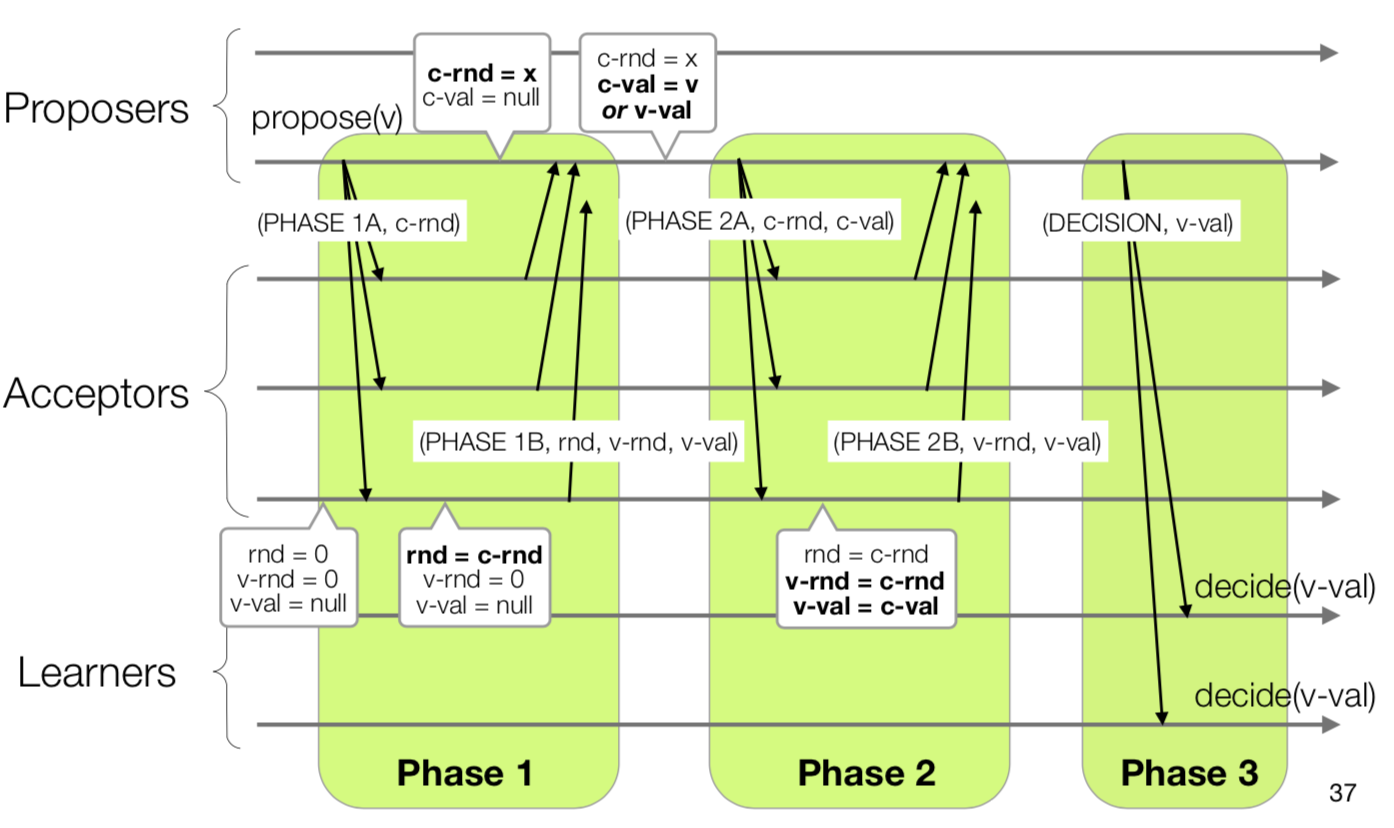
\includegraphics{img/paxos.png}
\caption[The architecture of the system]{ The architecture of the system. The
  \textit{Viper IDE} and \textit{Viper Debugger} boxes denote, respectively,
  the main Viper extension and the new debugger extension. They both interact,
  independently, with Visual Studio Code. Viper Server is responsible for
  running the verification backends.}
\label{fig:paxos}
\end{figure}

[should I add correctness, liveness, and so on?]

Remember that this algorithm allows only for the decision of one value; once value is decided, another instance of Paxos has to be initiated. Hence, for realistic use cases one would use system that allow to run multiple instances of paxos in a row, such as MultiPaxos.

The presented version of Paxos is the simplest one. Liveness in this case is not guaranteed; to ensure it, only the leader should be allowed to propose values, since otherwise it is possible that two proposers keep stealing their turn from each others without making any progress. Therefore the proposers should forward their values to the leader that will then try to propose them.

Various other improvements can be performed: for example, the leader could start phase 1 before a value is proposed, which means that once a value is ready to be proposed we can start directly from phase 2, virtually removing the delay of phase 1.
Also, at the end of Phase 2B the acceptors could send the decided value directly to the learners instead of having to first send it to the proposers; this allows to remove a whole message delay from the algorithm.

[should I write best message delays?]

\section{GeoPaxos}\label{sec:GeoPaxos}
Many current online services must serve clients distributed across geographic areas. In order to improve service avail- ability and performance, servers are typically replicated and deployed over geographically distributed sites (i.e., datacen- ters). By replicating the servers, the service can be configured to tolerate the crash of nodes within a single datacenter and the disruption of an entire datacenter. Geographic replication can improve performance by placing the data close to the clients, which reduces service latency.

Designing systems that coordinate geographically dis- tributed replicas is challenging. Some replicated systems resort to weak consistency to avoid the overhead of wide-area com- munication. Strong consistency provides more intuitive service behavior than weak consistency, at the cost of increased latency. Due to the importance of providing services that clients can intuitively understand, several approaches have been proposed to improve the performance of geo-distributed strongly consistent systems (e.g., [1], [2], [3], [4]). This paper presents GeoPaxos, a protocol that combines three insights to implement efficient state machine replication in geographically distributed environments.

First, GeoPaxos decouples ordering from execution [5]. Although Paxos introduces different roles for the ordering and execution of operations (acceptors and learners, respec- tively [6]), Paxos-based systems typically combine the two roles in a replica (e.g., [1], [2], [7]). Coupling order and execution in a geographically distributed setting, however, leads to a performance dilemma. On the one hand, replicas must be deployed near clients to reduce latency (e.g., clients can quickly read from a nearby replica). On the other hand, distributing replicas across geographic areas to serve remote clients slows down ordering, since replicas must coordinate to order operations. By decoupling order from execution, GeoPaxos can quickly order operations using servers in dif- ferent datacenters within the same region [1] and deploy geo- graphically distributed replicas without penalizing the ordering of operations.

Second, instead of totally ordering operations before execut- ing them, as traditionally done in state machine replication [8], GeoPaxos partially orders operations. It is well-known that state machine replication does not need a total order of operations [9] and a few systems have exploited this fact (e.g., [10], [2]). GeoPaxos differs from existing systems in the way it implements partial order. GeoPaxos uses multiple independent instances of Multi-Paxos [11] to order operations—hereafter, we call an instance of Multi-Paxos a Paxos group or simply a group. Operations are ordered by one or more groups, depending on the objects they access. Operations ordered by a single group are the most efficient ones since they involve servers in datacenters in the same region. Operations that involve multiple groups require coordination among servers in datacenters that may be far apart and thus perform worse than single-group operations. GeoPaxos’s approach to partial order can take advantage of public cloud computing infrastructures such as Amazon EC2 [12]: fault tolerance is provided by nodes in datacenters in different availability zones, within the same region; performance is provided by replicas in different regions. Although intra-region redundancy does not tolerate catastrophic failures in which all datacenters of a region are wiped out, most applications do not require this level of reliability [1].

Third, to maximize the number of single-group operations, GeoPaxos exploits geographic locality. Geographic locality presumes that objects have a preferred site, that is, a site where objects are most likely accessed. Geographic locality is common in many online services. For example, operations on a user’s data often originate in the region where the user is. Some distributed systems exploit locality by sharding the data and placing shards near the users of the data (e.g., [1], [4]). GeoPaxos does not shard the service state; instead, it distributes the responsibility for ordering operations to Paxos groups deployed in different regions. Operations are ordered by the groups in the preferred sites of the objects accessed by the operation.

The rest of the paper is structured as follows. Section II details the system model and recalls fundamental notions. Section III overviews the main paper contributions. Section IV
details GeoPaxos. Section V describes our prototype. Sec- tion VI presents our performance evaluation. Section VII reviews related work and Section VIII concludes the paper.

[add better explanations of the things]
[add images]